%!TEX root = ../main.tex

\subsection{Copula Dependency Measures} % (fold)
\label{sub:copula_dependency_measures}

By simulating 250000 weeks of shocks in the copula, and then transforming these shocks into standardized residuals for each of the factors, we can test copula's ability to generate the threshold correlations in the data. The results are given in~\autoref{fig:threshold_simulated1}. Again, we use the standardized returns of ARMA-GARCH models. We display patterns from constant copula models, as the dynamic models vary over time.

\begin{figure}[!ht]
  \centering
  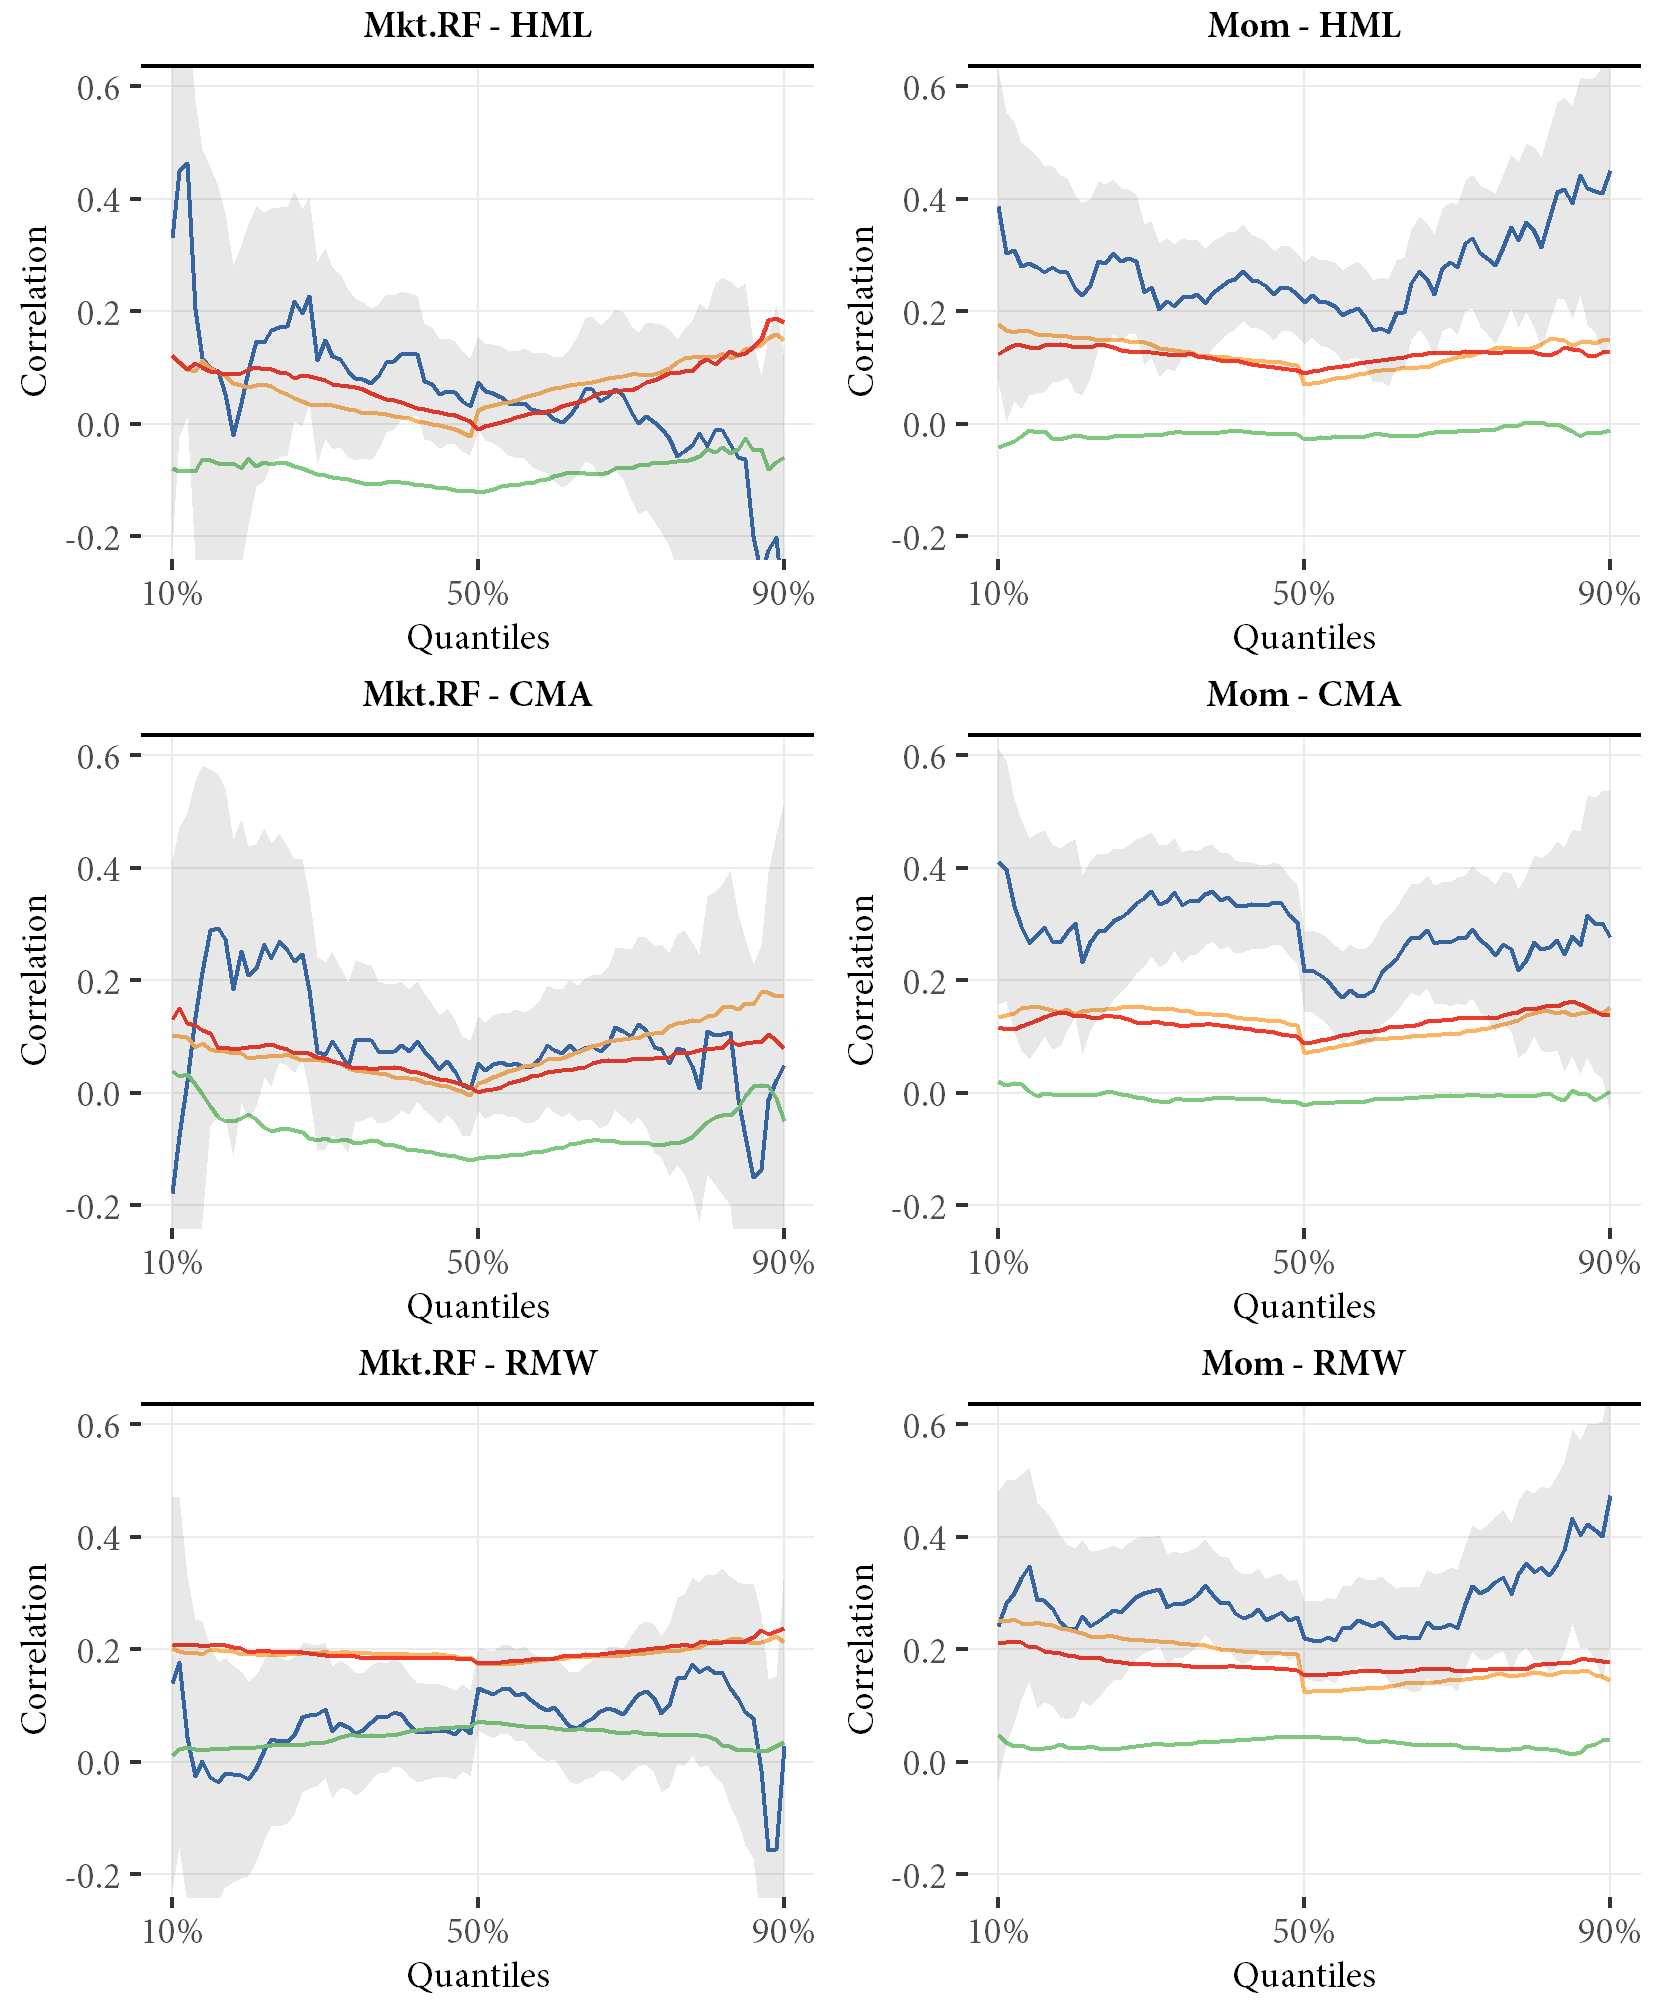
\includegraphics[scale=1]{graphics/threshold_simulated1.png}  

  \caption{Threshold correlations of simulated constant copula standardized returns, with ARMA-GARCH standardized returns (95\% confidence bounds taking the ARMA-GARCH models as given). The simulated threshold correlations are based on 250000 simulated returns each.}
  
  \label{fig:threshold_simulated1}
\end{figure}
\begin{figure}[!ht]
  \ContinuedFloat
  \centering

  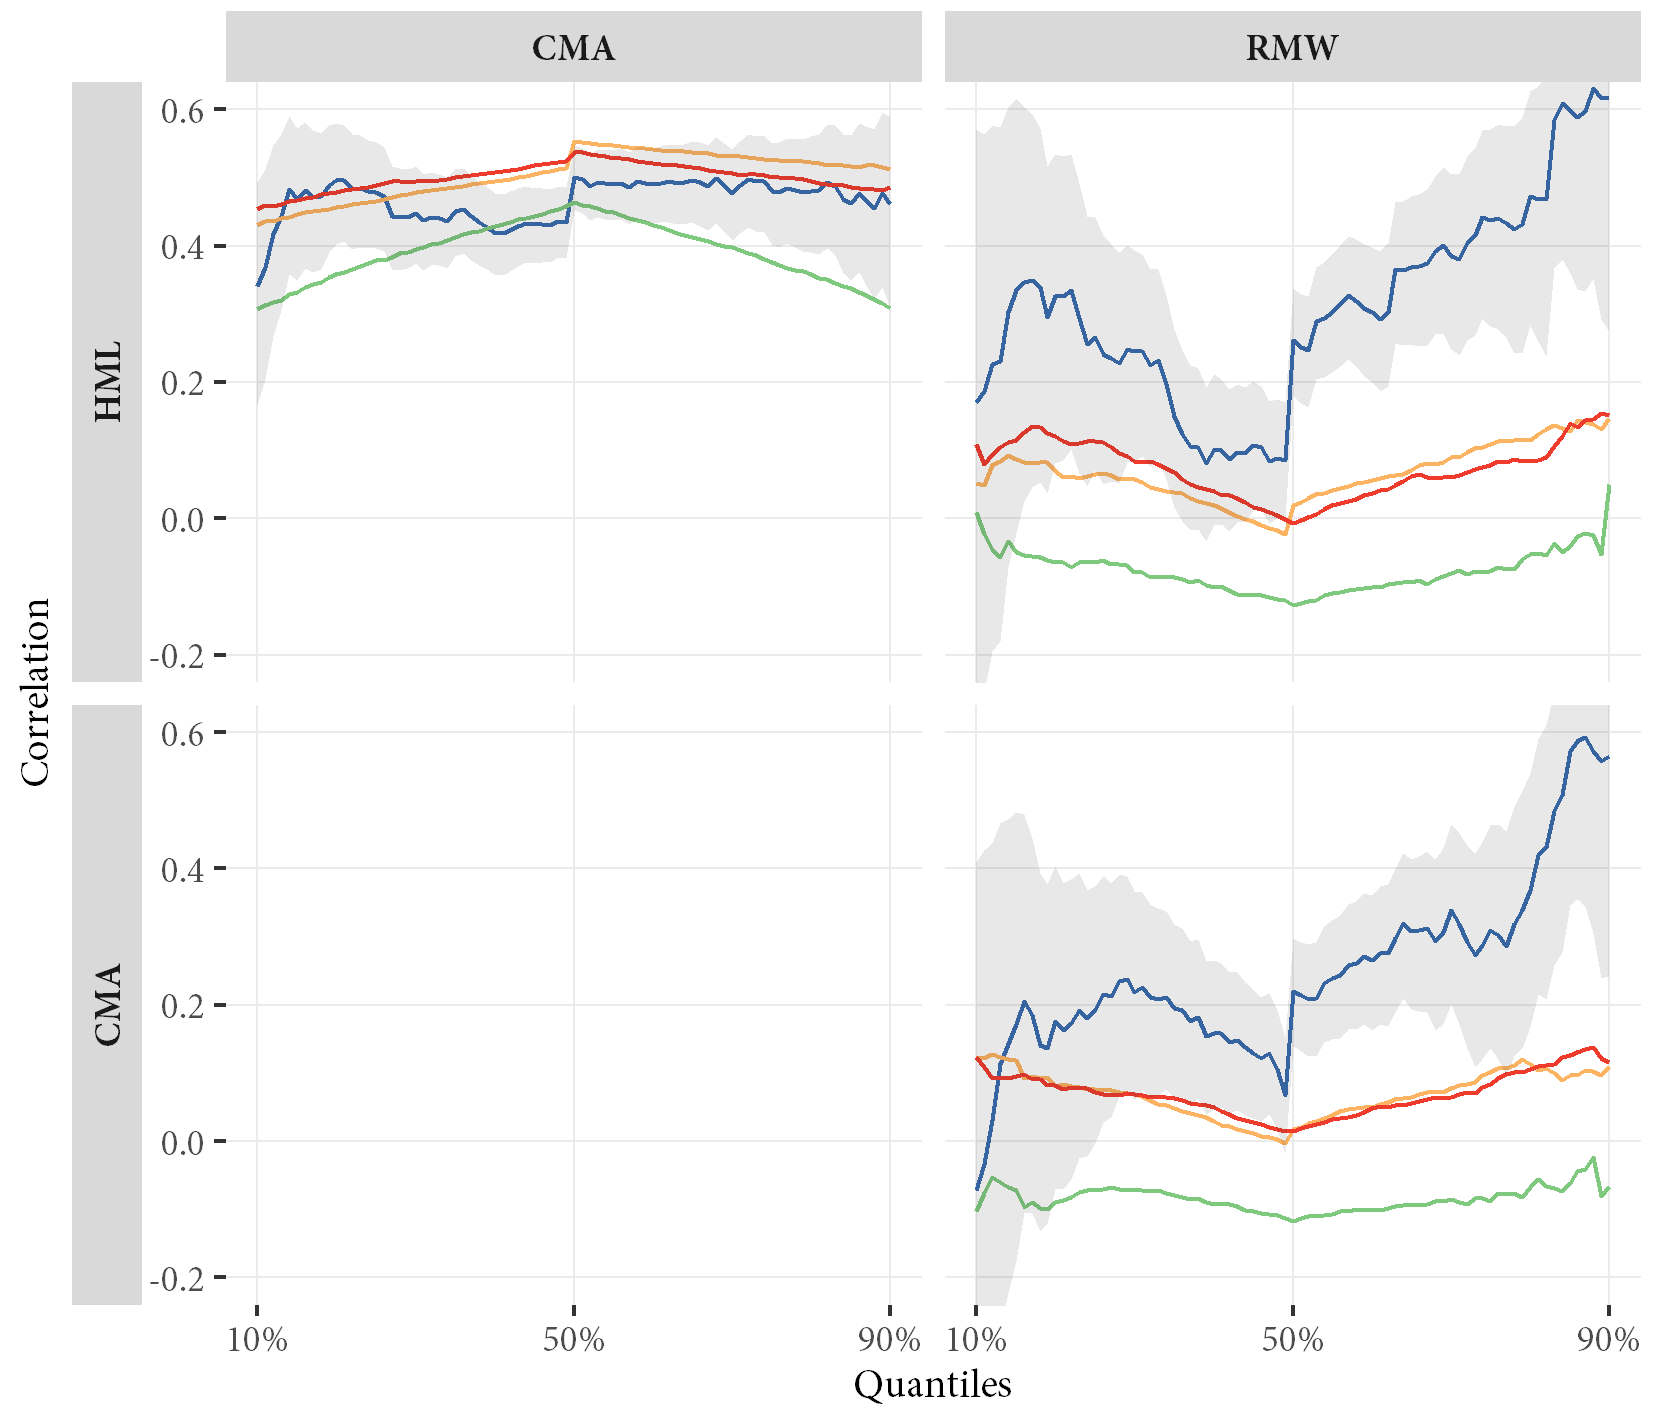
\includegraphics[scale=1]{graphics/threshold_simulated2.png}  

  \caption{Threshold correlations of simulated copula standardized returns (cont.)}
\end{figure}

First, we note that for most factors, the normal copula is the farthest away from generating threshold correlations that correspond to the empirical distribution around the median. More specifically, it seems to underestimate the threshold correlation, i.e. not generate sufficient tail dependence. The Student's \textit{t} and skewed Student's \textit{t} copulae better capture the threshold correlations, as the fatter tails of the Student's \textit{t} distribution allows for tail dependence. For example, note how the normal copula generates negative threshold correlations for both the Mom - HML and RMW - HML asset pairs, while the Student's \textit{t} based copulae are much closer to the higher values in the data. On the other hand, the Student's \textit{t} based copulae sometimes seem to overshoot the empirical threshold correlation, as in the Mkt-RF - RMW asset pair.

Second, we find that although the skewed Student's \textit{t} does generate some asymmetry around the mean, which can be seen most clearly for the Mom - RMW and RMW - HML asset pairs, the asymmetry is far too weak to be an accurate description of the data. 

In conclusion, threshold correlation comparison between empirical and simulated data shows the limitations of our copula approach. Although the copulae are flexible and can express tail dependence, which is a clear improvement to no tail dependence at all, it does not overlap very well with the data. For example, the Student's \textit{t} copula only has one degree of freedom parameter that controls the fatness of tails, and the skewed Student's \textit{t} copula only has one skewness parameter for each series. This imposes limits on how strongly the model can express fat tails or asymmetries between factors A and B and simultaneously express other fat tails or asymmetries (or lack thereof) between factors A and C. For a collection of six factors with heterogenous dependence, this is even harder. This is a clear limitation of the quite parsimonious copula approach, and will be discussed further in the concluding section. Although imperfect, the copula modeling of tail dependence could constitute a significant improvement to alternatives, especially in the field of risk management, where understanding of tail events is paramount.

% subsection copula_dependency_measures (end)
